\chapter{Background}

\section{Heart Disease}
	Heart disease is the leading cause of death for both adult men and women \cite{CDC2015}. The term "heart disease" refers to conditions that involve narrow or blocked blood vessels, which can lead to a heart attack, or conditions that affect the heart muscle, valves, or rhythm, which can lead to inefficient pumping and heart failure \cite{CDC2015}. In addition to adults, there are children who are born with congenital heart disease (CHD), heart defects that can be present at birth, and it's a growing problem that affects over 2 million people in the US \cite{Rosamond2007}. As surgical and treatment techniques have improved, children with CHD are living to adulthood. For both adults and children, in order to develop improved techniques for treatment and therapy, heart disease and cardiac function need to be accurately monitored.

\section{Standard Cardiac Magnetic Resonance Imaging (MRI) and Traditional Measures of Cardiac Function}
	Magnetic resonance imaging (MRI), a non-invasive, non-ionizing medical imaging technique, has become standard protocol for diagnosis, prognosis, and management of acquired and congenital heart diseases. Traditional measures of cardiac function, such as ventricular volumes, ventricular mass, and ejection fraction, can be derived from standard cardiac MRI. Whole heart function is typically assessed with these traditional metrics, but unfortunately, they may not contain enough information to explain the complex nature of some heart diseases. Moreover, there is a growing body of evidence that suggests that, when combined with clinical risk factors (e.g. hypertension), advanced measures of cardiac mechanics (e.g. cardiac strains and torsion) are better predictors of mortality compared to traditional measures \cite{Stanton2009} (Figure~\ref{fig:stanton}).

	\begin{figure}
		\centering
		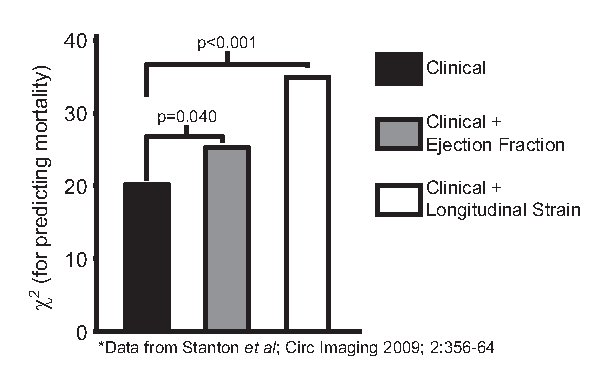
\includegraphics{figures/intro/stanton}
		\caption[Measuring cardiac strains dramatically improves the ability to predict mortality]{\textbf{Measuring cardiac strains dramatically improves the ability to predict mortality.}}
		\label{fig:stanton}
	\end{figure}

\section{Advanced Measures of Function: Cardiac Mechanics}
 	Cardiac mechanics, such as strain and torsion, measure the deformation of the heart as it contracts and relaxes throughout the cardiac cycle. Strain is a measure of how small segments of the myocardium shorten or lengthen during contraction and relaxation. In segments of the left ventricle, strain is commonly measured in three orthogonal directions: circumferential, radial, and longitudinal (Figure~\ref{fig:3D_strain_explanation}). Torsion is a measure the twisting motion along the longitudinal axis of the heart throughout the cardiac cycle. Cardiac mechanics can be quantified from analyzing the motion of small regions of the heart, which can be achieved by using an advanced imaging technique called spiral cine Displacement ENcoding with Stimulated Echoes (DENSE).
 	
 	\begin{figure}
 		\centering
 		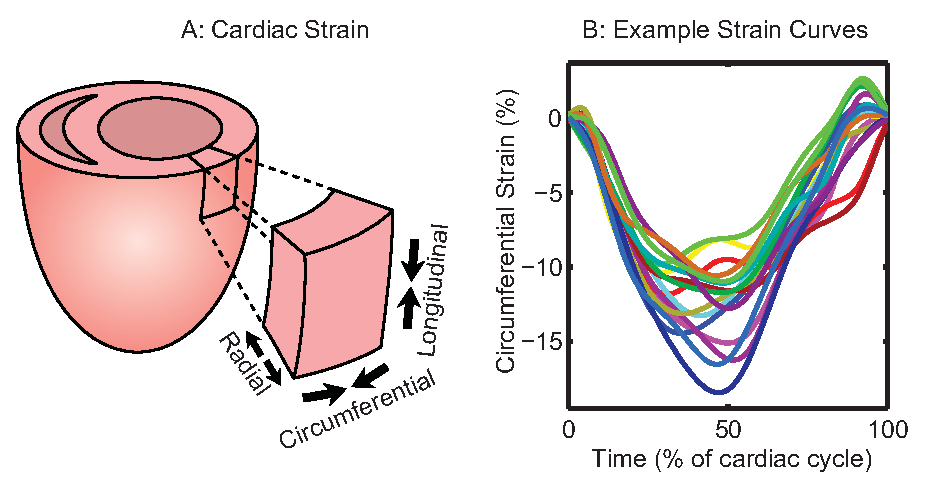
\includegraphics{figures/intro/3D_strain_explanation}
 		\caption[Strain analysis of myocardial segments in three orthogonal directions]{\textbf{Strain analysis of myocardial segments in three orthogonal directions.} A) Definition of the three orthogonal strain components: radial, circumferential, and longitudinal. B) Example circumferential strain curve over time throughout the cardiac cycle. Each curve represents the strain for a single myocardial segment. Negative values denote shortening.}
 		\label{fig:3D_strain_explanation}
 	\end{figure}

\section{Displacement Encoded Cardiac MRI}
	Spiral cine DENSE is an advanced cardiac magnetic resonance imaging technique that directly encodes the displacement of the myocardial tissue into the phase of the MR signal \cite{Aletras1999b}. Because of its quantitative nature, as opposed to qualitative such as in standard cardiac MRI, DENSE allows for simple and accurate quantification of cardiac mechanics. In addition, DENSE has good spatial resolution and good reproducibility \cite{Haggerty2013,Wehner2015a}. Moreover, DENSE has been used to quantify cardiac mechanics in both healthy and diseased animals and humans \cite{Aletras1999b,Aletras1999c,Kim2004,Ernande2012,Haggerty2013}

\section{Respiratory Motion and Blurring}
	Due to the heart's position resting on the diaphragm, breathing during CMR acquisition will result in respiratory image artifacts \cite{Axel1986}, which make images blurry and unusable (Figure~\ref{fig:good_bad_image_breathing_artifacts}). Thus, cardiac MR images are typically acquired using end-expiratory breath-holds, which are used to suspend respiration so the bulk motion of the heart is minimized during imaging. DENSE acquisitions are typically performed using end-expiratory breath-holds that are $\sim$15--20 s in duration \cite{Kim2004,Zhong2006a,Ernande2012,Zhong2010a,Aletras2005,Spottiswoode2007,Young2012c}. However, this method's success depends upon the patient's ability to breath-hold, which is limited in young subjects and many stages of advanced heart disease.
	
\section{Inconsistent Breath-holds}
	Unfortunately, patients typically struggle to achieve a consistent diaphragm position between successive breath-holds and variations of 4--13 mm are normal \cite{Liu1993,Wang1995a,Taylor1997a,Holland1998c,Fischer2006a}. Inconsistent breath-holds can impact the position of the heart with respect to the imaging plane (Figure~\ref{fig:range_of_diaphragm_position_breathing}). Peak strains vary along the longitudinal axis of the heart \cite{Kuijer2002,Moore2000,Young1994a,Feng2009,NasiraeiMoghaddam2010,Donekal2013a,Suever2017} and torsion is computed typically computed from two images acquired during \textit{separate} end-expiratory breath-holds \cite{Donekal2013a}. In both cases, quantification is performed assuming images were acquired at the same, consistent diaphragm position. Thus, we expect that translation of the heart with respect to the imaging plane (due to inconsistent end-expiratory positions) to result in differences and/or variability in measured strains and torsion. \textit{We hypothesized that this variability could be reduced by using a respiratory navigator to improve the consistency of the diaphragm position between breath-holds.}
	
	\begin{figure}
		\centering
		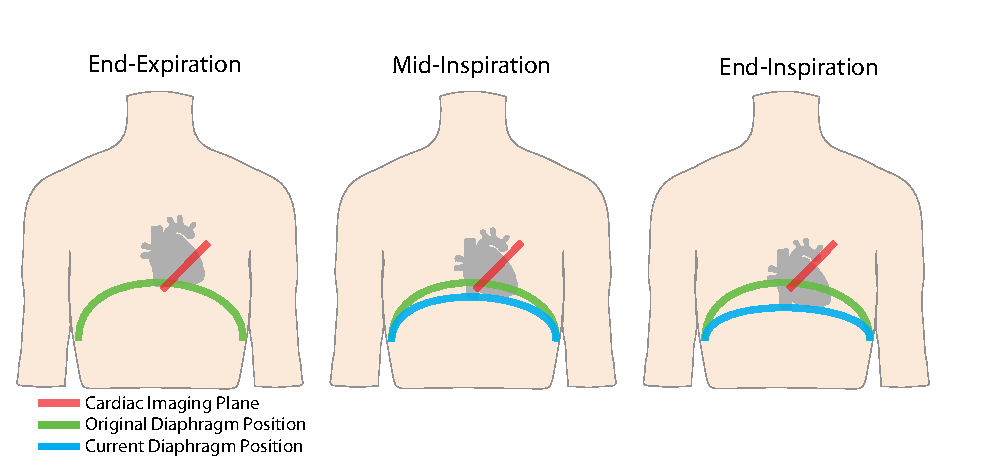
\includegraphics{figures/intro/range_of_diaphragm_position_breathing}
		\caption[During respiration, diaphragm motion causes the heart to translate a significant distance while the imaging plane remains fixed]{\textbf{During respiration, diaphragm motion causes the heart to translate a significant distance while the imaging plane remains fixed.}}
		\label{fig:range_of_diaphragm_position_breathing}
	\end{figure}
	
	\begin{figure}
		\centering
		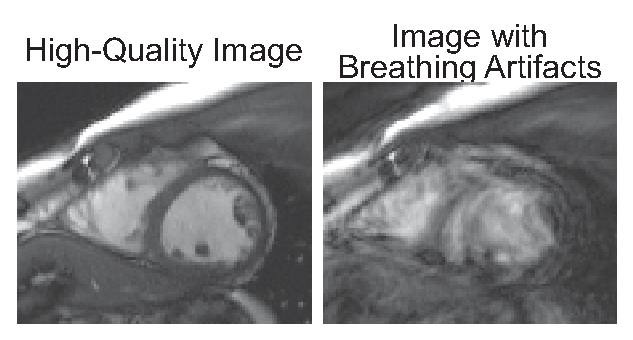
\includegraphics{figures/intro/good_bad_image_breathing_artifacts}
		\caption[High-quality image vs image with breathing artifacts that results in unusable data]{\textbf{High-quality image vs image with breathing artifacts that results in unusable data.}}
		\label{fig:good_bad_image_breathing_artifacts}
	\end{figure}

\section{Respiratory Navigator Gating}
	Respiratory navigator gating works by measuring the diaphragm position during normal breathing and only acquiring data when the diaphragm is within a pre-defined acceptance window (Figure~\ref{fig:navigator_gating_explanation}). Respiratory navigation is also used to overcome the limitations of short acquisitions (end-expiratory breath-holds), which limit the ability to acquire more robust data, such as high-resolution \cite{Wehner2014} or three-dimensional (3D) DENSE imaging \cite{Zhong2010a,Kar2014,Auger2012}. However, unlike other cardiac imaging techniques, the navigator echo in the DENSE sequence cannot occur at the beginning of the cardiac cycle as it would interfere with the displacement encoding. Instead, the navigator echo occurs immediately after data acquisition, at the end of the cardiac cycle, which creates several configurations as to how the navigator can be used to either accept or reject acquired DENSE data (prospective, retrospective, and dual). Previous studies have reported using prospective single navigator configuration \cite{Zhong2010a,Auger2012}. Each configuration has distinct advantages and disadvantages that can directly affect image quality and scan duration, but no formal comparison of the configurations has been performed. Moreover, the accuracy of derived cardiac mechanics and overall image quality for these navigator configurations compared with breath-hold acquisitions as a reference standard are largely unknown. \textit{Therefore, another goal of this study was to determine the optimal navigator configuration compared to breath-holds as a reference standard.}
	
\section{Navigator Efficiency}
	Navigator efficiency is defined as the total duration while the diaphragm is within the acceptance window versus the total scan duration. Unfortunately, due to poor navigator efficiency, respiratory navigator gating results in significantly increased scan duration. For example, previous CMR studies have reported respiratory navigator efficiencies of 20 to 45\% in adults [4–7] \cite{Abd-Elmoniem2011,Feuerlein2009,Jhooti2011,Wang1996}. This poor navigator efficiency lengthens the duration of currently used clinical imaging and limits clinical feasibility of emerging advanced imaging techniques.
	
	Navigator efficiency is typically poor because breathing patterns can be inconsistent \cite{Liu1993,Wang1995a,Taylor1997a}, as commonly seen in children, and the patient is generally unaware of the desired acceptance window location. The use of visual feedback of the diaphragm position during CMR has been shown to improve breathing consistency and efficiency in adults up to 29\% compared to traditional acquisitions without feedback \cite{Feuerlein2009,Jhooti2011}. Therefore, it's important to investigate whether similar benefits can be achieved using visual feedback with pediatric participants, which could have substantial clinical benefit. \textit{We hypothesized that engaging pediatric participants with a navigator controlled videogame to help control breathing patterns would improve navigator efficiency.}
	
	\begin{figure}
		\centering
		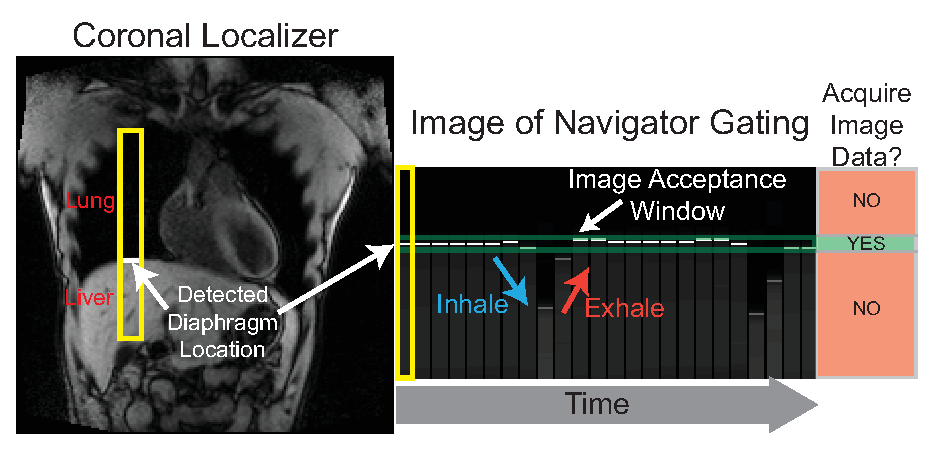
\includegraphics{figures/intro/navigator_gating_explanation}
		\caption[Respiratory navigator gating]{\textbf{Respiratory navigator gating.} (Left) The diaphragm is detected at the high-contrast interface between the lung (dark) and the liver (bright). (Right) The diaphragm location determined for multiple cardiac cycles with a narrow acceptance window	defining when image data was acquired.}
		\label{fig:navigator_gating_explanation}
	\end{figure}

\section{Dissertation Outline}
	The overall goal of this project was to optimize respiratory navigator gating, which would improve the clinical utility of DENSE. To accomplish this goal, we set out to 1) understand how respiratory navigator gating affects the reproducibility of measures of cardiac mechanics, 2) determine the optimal respiratory navigator configuration, and 3) improve navigator efficiency, which reduces scan duration, by using an interactive breathing-controlled videogame during cardiac MRI.
	
	\indent In Chapters 2 and 3, we address the effects of inconsistent end-expiratory diaphragm position between breath-holds and respiratory navigator gating on DENSE-derived cardiac mechanics, such as left ventricular strain and torsion. In Chapter 2, we learn that cardiac strain is insensitive to normal changes in end-expiratory position between breath-hold DENSE acquisitions. In Chapter 3, we discover that use of a respiratory navigator has the ability to significantly reduce the variability of cardiac torsion and thus the sample size needed to detect small changes in torsion. The conclusions of the studies performed for Chapters 2 and 3 discuss the importance of employing a respiratory navigator or some form of consistent respiratory compensation for future studies.
	
	\indent In Chapter 4, we determine the optimal navigator configuration compared to the breath-hold "gold-standard". Importantly, we learn that although strains were consistent between different navigator configurations and breath-holds. However, in terms of image quality, the dual navigator configuration was no different than breath-holds in adults and resulted in the best image quality in children. Unfortunately, the high image quality resulted in a trade off with navigator efficiency, which was the poorest for the dual navigator configuration compared to the other navigator configurations. The conclusion of chapter 4 discusses that some form of respiratory navigator feedback may be helpful in improving the poor navigator efficiency of the dual navigator.
	
	\indent In Chapter 5, we developed and tested an interactive breathing-controlled videogame to improve navigator efficiency. Fifty children participated in using the videogame during navigator-gated DENSE cardiac MRI. Analysis was performed to assess the videogame's effects on navigator efficiency, heart rate, and derived strain compared to normal free-breathing. We discovered that using the videogame during navigator-gated cardiac MRI resulted in a significant improvement in navigator efficiency. The conclusion of this chapter discusses that this form of navigator efficiency improvement should be generalizable to all cardiac MRI that employ a respiratory navigator.
	
	\indent In Chapter 6, we discuss a summary of the results of all these studies, their clinical implications, and future directions.

